\begin{figure}[H]
    \centering
    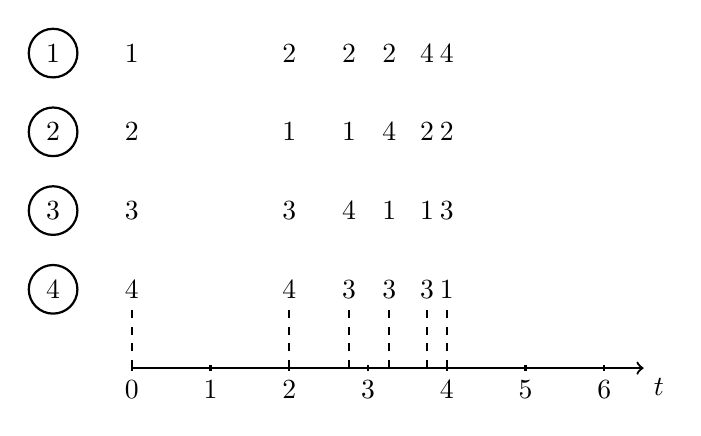
\begin{tikzpicture}[thick]
        \draw[thick,->] (0,0) -- (6.5,0) node[anchor=north west]
            {$t$};
%        \draw[thick,->] (0,0) -- (0,8) node[anchor=south east]
%            {valor$(t)$};
        \foreach \x in {0, 1,..., 6}
        \draw (\x cm,1pt) -- (\x cm,-1pt)
        node[anchor=north] {$\x$};
        \node[circle, draw] at (-1,1 cm) {$4$};
        \node[circle, draw] at (-1,2 cm) {$3$};
        \node[circle, draw] at (-1,3 cm) {$2$};
        \node[circle, draw] at (-1,4 cm) {$1$};

        \node at (0,1 cm) {$4$};
        \node at (0,2 cm) {$3$};
        \node at (0,3 cm) {$2$};
        \node at (0,4 cm) {$1$};

        \node at (2,1 cm) {$4$};
        \node at (2,2 cm) {$3$};
        \node at (2,3 cm) {$1$};
        \node at (2,4 cm) {$2$};

        \node at (2.76,1 cm) {$3$};
        \node at (2.76,2 cm) {$4$};
        \node at (2.76,3 cm) {$1$};
        \node at (2.76,4 cm) {$2$};

        \node at (3.27,1 cm) {$3$};
        \node at (3.27,2 cm) {$1$};
        \node at (3.27,3 cm) {$4$};
        \node at (3.27,4 cm) {$2$};

        \node at (3.75,1 cm) {$3$};
        \node at (3.75,2 cm) {$1$};
        \node at (3.75,3 cm) {$2$};
        \node at (3.75,4 cm) {$4$};

        \node at (4,1 cm) {$1$};
        \node at (4,2 cm) {$3$};
        \node at (4,3 cm) {$2$};
        \node at (4,4 cm) {$4$};


        \draw[dashed] (0, 0) -- (0, 0.8);
        \draw[dashed] (2, 0) -- (2, 0.8);
        \draw[dashed] (2.76, 0) -- (2.76, 0.8);
        \draw[dashed] (3.27, 0) -- (3.27, 0.8);
        \draw[dashed] (3.75, 0) -- (3.75, 0.8);
        \draw[dashed] (4, 0) -- (4, 0.8);


    \end{tikzpicture}
    \caption[Exemplo de trocas na lista ordenada]{Vetor com os índices dos elementos, ordenado
    pelos valores dos elementos no tempo $t = 0$ e suas
    alterações a medida que o tempo avança, para os quatro
    elementos da Figura~\ref{fig:ordenacao:exemplo}.}
    \label{fig:lista:vetores}
\end{figure}